\section{Cím}

Általános bevezető szöveg. A \ref{fig:child_dragged} ábrán látható ahogy egy robotraj együttesen elmozdít egy kislányt.

\begin{figure}[h]
    \centering
    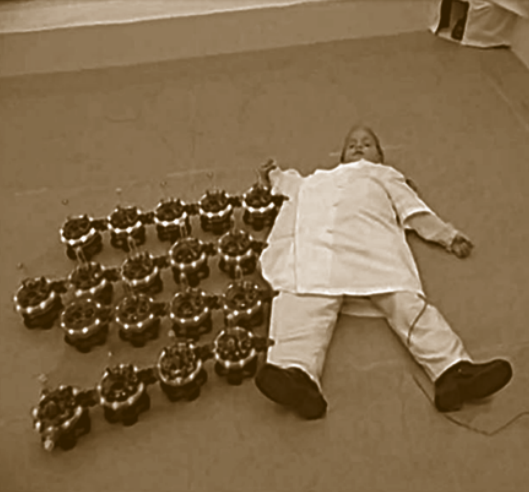
\includegraphics[scale=0.6]{figures/images/literature/child_dragged_robots.png}
    \caption{Rövid szöveg a képről, hivatkozás \cite{parker2016multiple}}
    \label{fig:child_dragged}
\end{figure}

\section{Cím 2}

Két ábra egymás mellett (lásd \ref{fig:insbots} ábra).

\begin{figure}[h]
    \centering
    \hfill
    \subfigure[Insbot \cite{colot2004insbot}]{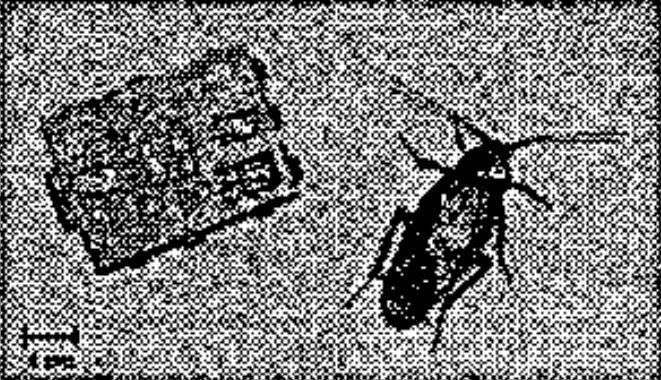
\includegraphics[scale=0.3]{figures/images/literature/insbot.png}}
    \hfill
    \subfigure[Insbot és csótányok interakciója \cite{garnier2011ants}.]{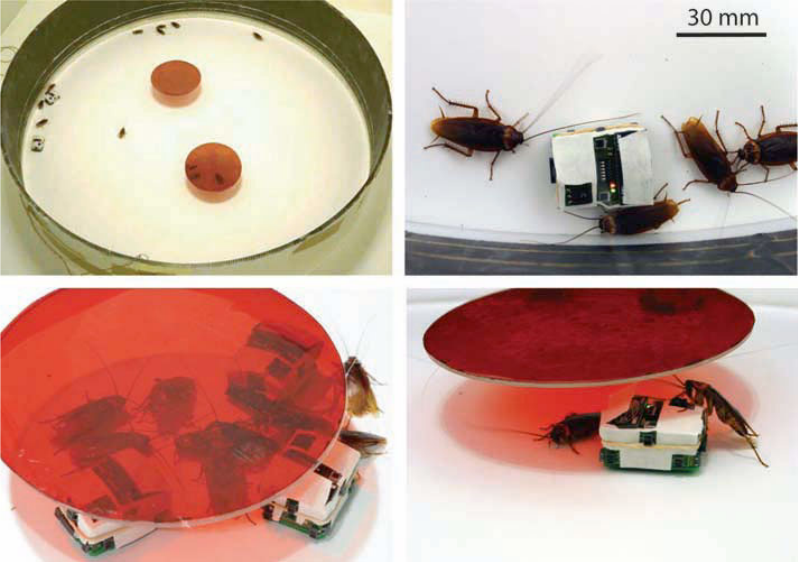
\includegraphics[scale=0.25]{figures/images/literature/insbot_cockroach.png}}
    
    \caption{Insbot és csótányok interakciója. Az insbot-ok képesek a csótányokat csalogatni.}
    \label{fig:insbots}
\end{figure}